\documentclass[a4paper]{book}
\usepackage{tocbibind} % for toc show inside pdf
\usepackage[
	%urlbordercolor = {1 1 1},
	%linkbordercolor = {1 1 1},
	%citebordercolor = {1 1 1},
    bookmarksnumbered, % add bookmark number in pdf output
	urlcolor = blue,
	colorlinks = true,
	citecolor = black,
	linkcolor = black]{hyperref}
\usepackage{graphicx}
\usepackage{xltxtra}
\usepackage{fancyhdr}
\usepackage{booktabs}
\usepackage{indentfirst}
\usepackage{framed,color}
\usepackage{footnpag}
\usepackage{array}
\usepackage[font=small,format=plain,labelfont=bf,up,textfont=it,up]{caption}
\usepackage[top=25mm,bottom=20mm,left=30mm,right=25mm]{geometry}

\usepackage{titlesec} % texlive-latex-extra package
\usepackage[titletoc]{appendix} % this is used for \appendices

\definecolor{colorchapter}{RGB}{70,130,180}     % SteelBlue
\definecolor{colorsection}{RGB}{95,158,160}    % CadetBlue
\definecolor{colorsubsection}{RGB}{139,0,0} % DarkRed
\definecolor{colorheader}{RGB}{70,130,180} % SteelBlue


\titleformat{\section}
{\color{colorsection}\normalfont\Large\bfseries}
{\color{colorsection}\thesection}{1em}{}
\titleformat{\subsection}
{\color{colorsubsection}\normalfont\large\bfseries}
{\color{colorsubsection}\thesubsection}{1em}{}

\definecolor{shadecolor}{gray}{0.90}

\setromanfont[Mapping=tex-text,BoldFont=Microsoft YaHei]{Microsoft YaHei}
\setmonofont{Microsoft YaHei}

\XeTeXlinebreaklocale{zh}
\XeTeXlinebreakskip=0em plus 0.1em minus 0.01em
\XeTeXlinebreakpenalty=0

\settowidth{\parindent}{文文}
\setcounter{footnote}{0}

\title{{跟我学STM8}}
\author{Larry Cai}

\makeatletter
\let\savedauthor=\@author
\let\savedtitle=\@title
\def\imgwidth{.6\linewidth}
\def\maxwidth{\ifdim\Gin@nat@width>\imgwidth\imgwidth
\else\Gin@nat@width\fi}
\makeatother

\title{\huge{\savedtitle}}

\author{\textbf{\savedauthor}\thanks{}}
\def\w3cdtfymd{\the\year-\ifnum\month<10 0\fi\the\month-\ifnum\day<10 0\fi\the\day}
\date{\w3cdtfymd}
%\renewcommand{\thefootnote}{\fnsymbol{footnote}}

\newcommand{\PreserveBackslash}[1]{\let\temp=\\#1\let\\=\temp}
\let\PBS=\PreserveBackslash
\makeatletter
  \setlength\headheight{12\p@}
  \setlength\headsep   {.25in}
  \setlength\topskip   {10\p@}
  \setlength\footskip{.35in}
  \setlength\textwidth{400\p@}
  
  \setlength\@tempdima{\paperheight}
  \addtolength\@tempdima{-2in}
  \divide\@tempdima\baselineskip
  \@tempcnta=\@tempdima
  \setlength\textheight{\@tempcnta\baselineskip}
  \addtolength\textheight{\topskip}
  
  \setlength\@tempdima        {\paperwidth}
  \addtolength\@tempdima      {-\textwidth}
  \setlength\oddsidemargin    {\paperwidth}
  \addtolength\oddsidemargin  {-2.35in}
  \addtolength\oddsidemargin  {-\textwidth}
  \setlength\marginparwidth   {0pt}
  \@settopoint\oddsidemargin
  \@settopoint\marginparwidth
  \setlength\evensidemargin  {\paperwidth}
  \addtolength\evensidemargin{-2.35in}
  \addtolength\evensidemargin{-\textwidth}
  \@settopoint\evensidemargin
  
  \setlength\topmargin{\paperheight}
  \addtolength\topmargin{-2in}
  \addtolength\topmargin{-\headheight}
  \addtolength\topmargin{-\headsep}
  \addtolength\topmargin{-\textheight}
  \addtolength\topmargin{-\footskip}     % this might be wrong!
  \addtolength\topmargin{-.5\topmargin}
  \@settopoint\topmargin
  %\@addtoreset{footnote}{page}  
\makeatother

%\fancypagestyle{plain}{\fancyhf{}\fancyfoot[LE,RO]{\footnotesize\textbf\thepage}}
\fancypagestyle{plain}{\fancyhf{}\fancyfoot{}} % make sure no page number in page of first chapter

\pagestyle{plain}


\renewcommand{\headrulewidth}{0pt}
\renewcommand{\footrulewidth}{0pt}
\renewcommand{\baselinestretch}{1.5}\normalsize

\newcounter{img}[chapter]
\renewcommand{\theimg}{\thechapter.\arabic{img}}
\newcommand{\img}[1]{\begin{figure}[h!]
	\refstepcounter{img}
	\label{img:\theimg}
	\centering\includegraphics[width=\maxwidth]{figures/\theimg.png}
	\caption{#1}
\end{figure}}

\newcounter{tab}[chapter]
\renewcommand{\thetab}{\thechapter.\arabic{tab}}

\newcommand{\prechap}{第}
\newcommand{\postchap}{章}
\newcommand{\presect}{}
\newcommand{\postsect}{节}
\renewcommand{\chaptermark}[1]{\markboth{\textbf{\prechap \thechapter \postchap}\hspace*{1ex}#1}{}}
\renewcommand{\sectionmark}[1]{\markright{\textbf{\presect \thesection \postsect}\hspace*{1ex}#1}}
\newcommand{\chap}[1]{\newpage\thispagestyle{empty}\chapter{#1}\label{chap:\thechapter}}
\newcommand{\chapref}[1]{\hyperref[chap:#1]{\prechap #1\postchap}}
\newcommand{\imgref}[1]{\hyperref[img:#1]{图 #1}}
\newcommand{\tabref}[1]{\hyperref[tab:#1]{表 #1}}
\newcommand{\e}[1]{$ \times 10^{#1}$}
\renewcommand{\contentsname}{目录}
\renewcommand{\figurename}{图 }
\renewcommand{\tablename}{表 }
\renewcommand{\appendixname}{}

% chapter 
\makeatletter
\def\@makechapterhead#1{%
  \vspace*{50\p@}%
  {\parindent \z@ \raggedright \normalfont
    \ifnum \c@secnumdepth >\m@ne
      \if@mainmatter
        \color{colorchapter}\normalfont\huge\bfseries\prechap{ }\thechapter{ }\postchap
        \par\nobreak
        \vskip 20\p@
      \fi
    \fi
    \interlinepenalty\@M
    \color{colorchapter}\normalfont\Huge\bfseries #1\par\nobreak
    \vskip 40\p@
  }}  
 
% this is for non-normal chapter like Acknownledgement, Preface, Contents  
\def\@makeschapterhead#1{%
  \vspace*{50\p@}%
  {\parindent \z@ \raggedright \normalfont
    \ifnum \c@secnumdepth >\m@ne
      \if@mainmatter
        \color{colorchapter}\normalfont\huge\bfseries \thechapter{ }
        \par\nobreak
        \vskip 20\p@
      \fi
    \fi
    \interlinepenalty\@M
    \color{colorchapter}\normalfont\Huge\bfseries #1\par\nobreak
    \vskip 40\p@
  }}  
\makeatother

\linespread{1.3}

\begin{document}
%\maketitle
\thispagestyle{empty}
\setcounter{tocdepth}{4}

\frontmatter
\chapter*{前言}
\addcontentsline{toc}{chapter}{前言}

说起这本手册的起因,是我去年6月做项目时上时碰到STM8这块芯片。这块芯片性能很强大,但是缺少对应的教材。当时我全靠着ST的英文文档,看得比较累。空下来就想,如果能有本教材就好了。毕设选题时,因为自己也做过一些研发类的项目,想换种形式,想到了这件事,就决定干脆自己写本教材。 但最后决定写成手册的形式,是因为一篇大牛的博客。这位大牛自身的技术积淀已经很强了,网上最流行的中文makefile教程就是他写的。他写的博文我经常看,感觉很有深度。据说很多出版社找他请他出书,但是他拒绝了,他说了这么一句话:“45岁之前绝不出书”,因为他觉得只有到了那个时候,自己才可能得到足够的积淀,才可能出的了精品。看到这句话,我想以我的能力又怎敢称之为教材呢?还是叫它手册吧。 在惠普以及爱立信的实习过程中,我接触了很多软件方面好用的工具,成熟的软件工程思想。比如说git,就是非常好的版本控制管理软件,比如说agile,消除了传统软件开发过程中的部分问题。我觉得,软件开发中的诸多问题,随着编程规模的扩大,参与人数的增多,在硬件开发中也会逐步地体现出来。所以,这些工具及思想方式引入到嵌入式编程,将是一种趋势。本手册亦不指望能够引领什么潮流,只希望能对STM8的学习者,有一个有益的指导,仅此而已。

\subsection*{适合的对象}

本手册适合具有C语言功底,并能在51或AVR上进行简单程序设计的单片机爱好者。如果没有C语言基础的,推荐\href{http://product.china-pub.com/14975\&ref=browse}{《C程序设计语言》},没有单片机基础的,本手册建议从马潮教授编写的\href{http://www.amazon.cn/AVR\%E5\%8D\%95\%E7\%89\%87\%E6\%9C\%BA\%E5\%B5\%8C\%E5\%85\%A5\%E5\%BC\%8F\%E7\%B3\%BB\%E7\%BB\%9F\%E5\%8E\%9F\%E7\%90\%86\%E4\%B8\%8E\%E5\%BA\%94\%E7\%94\%A8\%E5\%AE\%9E\%E8\%B7\%B5-\%E9\%A9\%AC\%E6\%BD\%AE/dp/B005GZQWB0/ref=sr\_1\_1?ie=UTF8\&qid=1335097650\&sr=8-1}{《AVR单片机嵌入式系统原理与应用实践(第2版)》}

\section*{本书结构}

\begin{itemize}\setlength{\itemsep}{1pt}\setlength{\parskip}{0pt}\setlength{\parsep}{0pt}
\item[*]
  第一章:前言
\item[*]
  第二章:重读C语言
\item[*]
  第三章:软件开发那点事
\item[*]
  第四章:STM8芯片资源简介
\item[*]
  第五章:STM8官方软件库简介
\item[*]
  第六章:STM8S编程实战
\end{itemize}
\subsection*{封面及封底}

因为喜欢排版,就自己设计了一个。封面封底的图片都是我本人在华东师范大学的校园里自行拍摄的,使用COREDRAW,进行后期处理。

\subsection*{项目地址}

本次STM8学习项目托管在github上,并且项目完全开源。欢迎大家访问:\href{www.github.com/vincent5295/stm8teach}{www.github.com/vincent5295/stm8teach}。

\section*{一些注意事项}

\subsection*{本手册的是如何写作的}

本手册基于markdown格式,我在我的一台上网本(ubuntu)和两台工作站(windows\&vista)上分别安装了gedit,相对于notepad++,gedit对markdown的语法高亮支持最好,使用起来很舒服。编辑完后使用\href{www.github.com/larrycai/mkbok}{mkbok程序}进行相应tex、pdf、epub等格式文件的生成。

\subsection*{如何阅读本手册}

一般来说,建议直接阅读电子版,一来可以获得较好的阅读体验,二来可以节约纸张。从保护视力的角度出发,自行打印纸质版也是可以的。但请一定不要忽视电子版,文中随处的可见的链接,是一笔宝贵的财富。本手册编写的一大准则,就是以自身为骨架,通过这些链接,能让读者得到丰富的内容。

\subsection*{你不能从本手册中获得}

本手册不是官方数据手册的汉化并堆砌,故详细的硬件寄存器资源及软件库函数说明并不能从中得到。手册本身不需实现盈利,故针对某开发板的内容在手册上也不能获得。同样关于程序语言的章节也不会提供过多C语言的细节。但以上这些在相关章节都会提到相应资源的方法,并且提供经验上的参考。

\subsection*{项目网站上的开发板}

项目网站上的核心板、资源板基于开放式设计。只是一个参考,如果不愿意自己画板子,可以直接将网站上的板子发到制版厂做,或者在网上买一款开发板都是可行的。资源板只提供原理图(因为模块太多,都做板子不实惠),因为这些模块PCB设计比较简单,需要做PCB的,自行copy所需模块,导入至PCB文件,连少许线即可。

\section*{致谢}

在本手册的编写过程中,遇到很多困难。在此感谢惠普以及爱立信的同事在软件编程方面对我的指点。特别要感谢爱立信中国通讯有限公司为期一周的敏捷开发培训,学到了不少有趣的东西。感谢larrycai在Github上的\href{www.github.com/larrycai/kaiyuanbook}{kaiyuanbook}以及\href{www.github.com/larrycai/mkbok}{mkbok}项目,为本手册的快速写作奠定了基础。最后要感谢周围的老师同学们在本项目的实践过程中,对本人给予的无私帮助,没有你们的鼓励与支持,就没有这本手册。

\tableofcontents\newpage\thispagestyle{empty}

% customize header & footer

\fancyhf{}
\fancyhead[LE]{\color{colorheader}\quad\small\textbf\thepage\quad\quad\small\leftmark}
\fancyhead[RO]{\color{colorheader}\small\rightmark\quad\quad\small\textbf\thepage\quad}
%\fancyhead[RE,LO]{\color{colorheader}\small{\savedtitle}} % book title 
%\fancyfoot[LE,RO]{\small\textbf\thepage} % page number
%\fancyfoot[C]{\small\textbf{hello}} % could add release information

%\renewcommand{\headrulewidth}{0.4pt}  % add one line
%\renewcommand{\headrule}{\color{red}} % conflict with headrulewidth
\pagestyle{fancy}

\mainmatter
\chap{重读C语言}

\section{C语言的那些事}

C语言是各大高校学习编程的入门语言。但作为入门语言,并不表示它是简单的。C语言的诞生是和UNIX操作系统密切相关的(一般说来,如果没用过UNIX/类UNIX操作系统,几乎不能认为那个人懂计算机),历史上很难分清到底是先有UNIX还是现有C(有点像先有鸡还是先有蛋的问题)。C语言是最接近底层特性的高级语言,但比汇编语言要好用地多。之前因为CPU编程空间的限制,人们迫不得已采用汇编进行编程。现在,在ARM的平台上已经能够获得C++的编译支持。STM8也有人专门做了程序的C++封装。不过现在嵌入式平台上的C++实现也颇有点像几十年前的C++,即C with class,着重使用类特性。事实上,PC上的C++语言经过这几十年来的发展,已经变得很不一样了。

下面两篇博文,可以用来检验自己C语言是否真正掌握。地址分别是\url{http://coolshell.cn/articles/945.html},还有\url{http://coolshell.cn/articles/873.html},希望他们能给你带来深入的思考\footnote{当然,如果今后要走程序员的道路,类似的这些问题在今后的面试中一定能碰得到(无论是别人面你还是你面别人)。}。

以下是从上述两篇博文中摘出来的5个问题,答案我会直接列在第五个问题后面,至于为什么,自己去网站找吧!Enjoy it!

1.下面的程序会输出什么?

{\footnotesize\begin{shaded}\begin{verbatim}
    #include <stdio.h>
    int main() 
    {
        float a = 12.5;
        printf("%d\n", a); 
        printf("%d\n", (int)a); 
        printf("%d\n", *(int *)&a); 
        return 0; 
    }
\end{verbatim}\end{shaded}}
2.下面,我们再来看一个交叉编译的事情,下面的两个文件可以编译通过吗?如果可以通过,结果是什么?

file1.c

{\footnotesize\begin{shaded}\begin{verbatim}
    int arr[80]; 
\end{verbatim}\end{shaded}}
file2.c

{\footnotesize\begin{shaded}\begin{verbatim}
extern int *arr;
int main() 
{
    arr[1] = 100;
    printf("%d\n", arr[1]);
    return 0; 
} 
\end{verbatim}\end{shaded}}
3.请问下面的程序输出什么?

{\footnotesize\begin{shaded}\begin{verbatim}
    #include <stdio.h> 
    int main() 
    {
    int i;
    i = 10;
    printf("i : %d\n",i);
    printf("sizeof(i++) is: %d\n",sizeof(i++));
    printf("i : %d\n",i);
    return 0; 
}
\end{verbatim}\end{shaded}}
4.下面这个函数返回值是什么?

{\footnotesize\begin{shaded}\begin{verbatim}
int x = 5;
int f() {
  int x = 3;
  {
    extern int x;
    return x;
  }
}
\end{verbatim}\end{shaded}}
5.下面的语句哪些是合法的?

{\footnotesize\begin{shaded}\begin{verbatim}
int (*pf)(void);
int f(void)
{

   pf = &f; // 没问题
   pf = ***f; // 取址?
   pf(); // 函数指针可以调用?
   (****pf)();  // 这又是什么?
   (***************f)(); // 这个够变态了吧?
}
\end{verbatim}\end{shaded}}
下面是答案:

第一题:

{\footnotesize\begin{shaded}\begin{verbatim}
0
12
1095237632
\end{verbatim}\end{shaded}}
第二题:

{\footnotesize\begin{shaded}\begin{verbatim}
该程序可以编译通过,但运行时会出错。
\end{verbatim}\end{shaded}}
第三题:

{\footnotesize\begin{shaded}\begin{verbatim}
10,4,10
\end{verbatim}\end{shaded}}
第四题:

{\footnotesize\begin{shaded}\begin{verbatim}
5
\end{verbatim}\end{shaded}}
第五题:

{\footnotesize\begin{shaded}\begin{verbatim}
全部合法。
\end{verbatim}\end{shaded}}
C语言不乏一些蛋疼的比赛,去看看\href{http://www0.us.ioccc.org/years.html}{国际C语言混乱代码大赛}吧,你能看到这样的代码\footnote{不用怀疑这段程序是否能够通过编译,这是一个图像降采样的工具。具体使用说明参见\url{http://www0.us.ioccc.org/2011/akari/hint.text}。我想说的是,维护这样的代码真是坑爹啊!}:

{\footnotesize\begin{shaded}\begin{verbatim}
	                               /*
	                              +
	                             +
	                            +
	                            +
	                            [         >i>n[t
	                             */   #include<stdio.h>
	                /*2w0,1m2,]_<n+a m+o>r>i>=>(['0n1'0)1;
	             */int/**/main(int/**/n,char**m){FILE*p,*q;int        A,k,a,r,i/*
	           #uinndcelfu_dset<rsitcdti_oa.nhs>i/_*/;char*d="P%"   "d\n%d\40%d"/**/
	         "\n%d\n\00wb+",b[1024],y[]="yuriyurarararayuruyuri*daijiken**akkari~n**"
	  "/y*u*k/riin<ty(uyr)g,aur,arr[a1r2a82*y2*/u*r{uyu}riOcyurhiyua**rrar+*arayra*="
       "yuruyurwiyuriyurara'rariayuruyuriyuriyu>rarararayuruy9uriyu3riyurar_aBrMaPrOaWy^?"
      "*]/f]`;hvroai<dp/f*i*s/<ii(f)a{tpguat<cahfaurh(+uf)a;f}vivn+tf/g*`*w/jmaa+i`ni("/**
     */"i+k[>+b+i>++b++>l[rb";int/**/u;for(i=0;i<101;i++)y[i*2]^="~hktrvg~dmG*eoa+%squ#l2"
     ":(wn\"1l))v?wM353{/Y;lgcGp`vedllwudvOK`cct~[|ju {stkjalor(stwvne\"gt\"yogYURUYURI"[
     i]^y[i*2+1]^4;/*!*/p=(n>1&&(m[1][0]-'-'||m[1][1]  !='\0'))?fopen(m[1],y+298):stdin;
      /*y/riynrt~(^w^)],]c+h+a+r+*+*[n>)+{>f+o<r<(-m]    =<2<5<64;}-]-(m+;yry[rm*])/[*
       */q=(n<3||!(m[2][0]-'-'||m[2][1]))?stdout /*]{     }[*/:fopen(m[2],d+14);if(!p||/*
       "]<<*-]>y++>u>>+r >+u+++y>--u---r>++i+++"  <)<      ;[>-m-.>a-.-i.++n.>[(w)*/!q/**/)
    return+printf("Can "  "not\x20open\40%s\40"    ""       "for\40%sing\n",m[!p?1:2],!p?/*
  o=82]5<<+(+3+1+&.(+  m  +-+1.)<)<|<|.6>4>-+(>    m-        &-1.9-2-)-|-|.28>-w-?-m.:>([28+
 */"read":"writ");for  (   a=k=u= 0;y[u];  u=2    +u){y[k++   ]=y[u];}if((a=fread(b,1,1024/*
,mY/R*Y"R*/,p/*U*/)/*          R*/ )>/*U{  */   2&& b/*Y*/[0]/*U*/=='P' &&4==/*"y*r/y)r\}
*/sscanf(b,d,&k,& A,&           i,  &r)&&        !   (k-6&&k -5)&&r==255){u=A;if(n>3){/*
]&<1<6<?<m.-+1>3> +:+ .1>3+++     .   -m-)      -;.u+=++.1<0< <; f<o<r<(.;<([m(=)/8*/
u++;i++;}fprintf   (q,    d,k,           u      >>1,i>>1,r);u  = k-5?8:4;k=3;}else
  /*]>*/{(u)=/*{   p> >u  >t>-]s                >++(.yryr*/+(    n+14>17)?8/4:8*5/
     4;}for(r=i=0  ;  ;){u*=6;u+=                (n>3?1:0);if    (y[u]&01)fputc(/*
      <g-e<t.c>h.a r  -(-).)8+<1.                 >;+i.(<)<     <)+{+i.f>([180*/1*
      (r),q);if(y[u   ]&16)k=A;if                               (y[u]&2)k--;if(i/*
      ("^w^NAMORI; {   I*/==a/*"                               )*/){/**/i=a=(u)*11
       &255;if(1&&0>=     (a=                                 fread(b,1,1024,p))&&
	")]i>(w)-;} {                                         /i-f-(-m-M1-0.)<{"
	 [ 8]==59/* */                                       )break;i=0;}r=b[i++]
	    ;u+=(/**>>                                     *..</<<<)<[[;]**/+8&*
	    (y+u))?(10-              r?4:2):(y[u]         &4)?(k?2:4):2;u=y[u/*
	     49;7i\(w)/;}             y}ru\=*ri[        ,mc]o;n}trientuu ren (
	     */]-(int)'`';}             fclose(          p);k= +fclose( q);
	      /*] <*.na/m*o{ri{                       d;^w^;}  }^_^}}
	       "   */   return  k-                -1+   /*\'   '-`*/
	             (   -/*}/   */0x01        );       {;{    }}
	                    ;           /*^w^*/        ;}
\end{verbatim}\end{shaded}}
\section{声明与定义}

\section{关于union}

\section{悬垂else}

\section{static的作用}

\section{断言之美}

关于进一步学习C语言的资料,我这里推荐下列三本书:\href{http://product.china-pub.com/14975\&ref=browse}{《C程序设计语言》}、{[}《C专家编程》{]}http://product.china-pub.com/38005)、\href{http://product.china-pub.com/38125}{《C陷阱与缺陷》}。一般来说,以《C程序设计语言》为基础,然后凭借后面两本书,知道C语言平时使用中一些容易犯错的地方。当然,如果你觉得还不够的话,以下这篇文章可能会适合你:\href{http://coolshell.cn/articles/4102.html}{如何学好C语言}。

\chap{软件开发那点事}

下面这些东西,是我在软件方面的书籍和实践中学习到的一点心得.之前学习嵌入式的时候,并没有接触到相关的知识.

\section{使用版本控制管理工具}

你是否有这样一种经历?当你在电脑上辛辛苦苦赶项目,马上就要做完了,但是因为突发情况(比如停电什么的),一瞬间,所有的工作都得从头开始,你欲哭无泪。于是,在几次这样的悲剧发生后,你吸取了教训,开始备份。比较原始的备份策略\footnote{一般有备份意识的人还是少的,本人即使在保持备份的意识下,也曾经因为一些原因丢失工作数据,造成一些尴尬情况的。}就是本工作文件定期复制到某个文件夹中,但过不久你就会发现,你已经分不清哪个是你最新版本的工作文件了。接着你以\emph{《文件名\_编辑时间》}的方式,把文件存放在同一路径下,这样似乎好一些了,但是如果整个硬盘遭受物理性损坏,所有备份的数据就一起陪葬了。似乎raid是一个好的解决方案,但是对于一般用户来说似乎又不太能够承受,而且,过于复杂的操作,会降低用户备份的积极性。可能你每天修改3、4次文件,但是却半个月才想到要备份一次。

那么什么是这个问题的优秀解决方案?回答是版本控制软件。他们具有对数据的存储、追踪、回退等诸多功能,方便好用。并且,github、google code等网站,有着高可靠的硬件支撑,为数据的安全性、可靠性,提供了有利的保证。通过其提供的免费或者付费服务,可以使用各种版本控制软件,如CVS、SVN、Git\ldots{}\ldots{}能够在对你的代码、数据进行方便管理的同时,保证安全性。

\subsection{使用Git来管理你的项目}

Git的优势在于快速、免费,当然,最终要的是,Git是分布式的,也就是说软件库是保存在用户本地,而非像clearcase、SVN这样,保存在远程服务器上。这样,就方便用户能够随时接触到代码。而且万一远程服务器出现故障,利用用户的数据也能基本恢复服务端的数据,数据的安全性更有保障。现在很多项目已经转移到Git上了,著名的有:\href{https://github.com/torvalds/linux}{linux内核},\href{https://github.com/groovy/groovy-core}{groovy},\href{https://github.com/jgm/pandoc}{pandoc}等等\ldots{}\ldots{}

如果你想学习Git,建议你在Github上建立一个账户。Github是一个支持Git的项目托管网站。有很多程序员使用该网站对自己的项目进行管理,并且与网友协作开发。价格方面,如果你的项目是开源的,那么一切都是免费的。

如果是第一次安装,配置环境的图文教程可以在\url{http://help.github.com/win-set-up-git/}找到。同时\href{http://help.github.com/}{Github的帮助网站}上面有关于Git的详细帮助。

当然如果需要系统的学习,\href{http://progit.org/}{《PROGIT》}这本书就是一个比较详尽的教程。

\section{说说IDE}

平时经常可以听到IDE,这个名字。那么IDE到底是什么呢? IDE的全称是: \textbf{I}ntegrated \textbf{D}evelopment \textbf{E}nvironment。我们平时写程序,无外乎编辑------编译------连接的过程,出故障了也许要做软/硬件单步调试。IDE给我们写程序,提供了上面这个流程中,所需要的一切。51上的KEIL,AVR上的ICC、CVAVR、IAR,都是IDE。

\subsection{IDE的优势}

我们大量使用IDE,是有原因的: 一方面IDE的安装使用极其方便,网上下好一路next即可,所有需要的工具都在里面,不许要用户自行去寻找。另一方面,IDE所提供的程序经过较好的测试,稳定性更高些。

\subsection{尝试着脱离IDE吧}

尽管IDE非常方便,但是我们

\section{对开源本身的思考}

\section{关于Makefile}

\section{其它参考}

\chap{STM8芯片简介}

\section{STM8的优势}

STM8S是意法半导体推出的一款8位高性能单片机。它基于哈弗结构,指令与数据存储空间分开,指令与数据可以同时存取,因而具有更高的执行效率。与AVR、51单片机比较,STM8拥有更为丰富的外设,更强大的主频、更优秀的特性。更重要的是,STM8供货稳定,性价比高。其中高端的STM8S208MB也就15元,低端的STM8S103F2系列一般也就2、3元左右,而AVR高端的mega128价格就在20元左右,且性能只能勉强赶得上ST的中端产品。更重要的是,STM8的编程方法与ST的高端产品,cortexM3市场的主流:STM32极其相似(但更简单点)。这种相似,给我们后来升级到STM32奠定了基础,要知道STM32最高端的F4系列具有150Mhz的主频,这样的升级,可以大大提升我们以后做应用的范围。

\section{STM8编程------寄存器or库函数?}

和STM32一样,历来STM8存在两种编程方式:寄存器直接编程和库函数编程。寄存器的优势在于,这样的编程方法和传统的8位单片机编程方法较一致,初学者容易适应,而且普遍认为寄存器编程的人不容易出错,程序执行效率较高。库函数的优势在于程序员开发效率高,ST将一些常用的方法封装起来,这样寄存器开发者几句话(可能还得经常查手册找参数)才能搞定的事情,库函数直接一个函数就搞定了,而且所有的参数设定都可以在库函数附带的使用手册中找到,方便快捷。 事实上,因为开发效率在实际应用中往往起着决定性的作用,比如大家同样做一个新产品,只有第一个做出来的才能在很早的时候抢占市场。等市场有了,在对产品维护的过程中优化程序运行效率。同时,使用库函数的方式能更好适应以后STM32,甚至DSP、ARM的编程方式。基于上述两个原因,本手册建议使用库函数编程方式。

\section{芯片资源简介}

一般来说,学习的时候可以用芯片功能强大一点,具体开发产品的时候可以根据官方给的\href{http://www.st.com/internet/com/SALES\_AND\_MARKETING\_RESOURCES/MARKETING\_COMMUNICATION/MARKETING\_BROCHURE/brstm8.pdf}{选型指南},来选择对应的芯片。本手册选用的是STM8S208MB芯片,它具有: \emph{最大24Mhz的运行速率}80个引脚(其中68个可用作IO引脚) \emph{37个外部中断引脚}128K可编程Flash,2MB的EEPROM \emph{6KB的RAM}并拥有CAN总线接口\ldots{}\ldots{} 具体资源可以从STM8S208MB的\href{http://www.st.com/internet/com/TECHNICAL\_RESOURCES/TECHNICAL\_LITERATURE/DATASHEET/CD00197787.pdf}{数据手册}获取,该芯片的APPLICATION NOTES、PROGRAMMING MANUALS、REFERENCE MANUALS等信息,可以从\href{http://www.st.com/internet/mcu/product/190232.jsp}{芯片的主页}下载。

\begin{figure}[htbp]
\centering
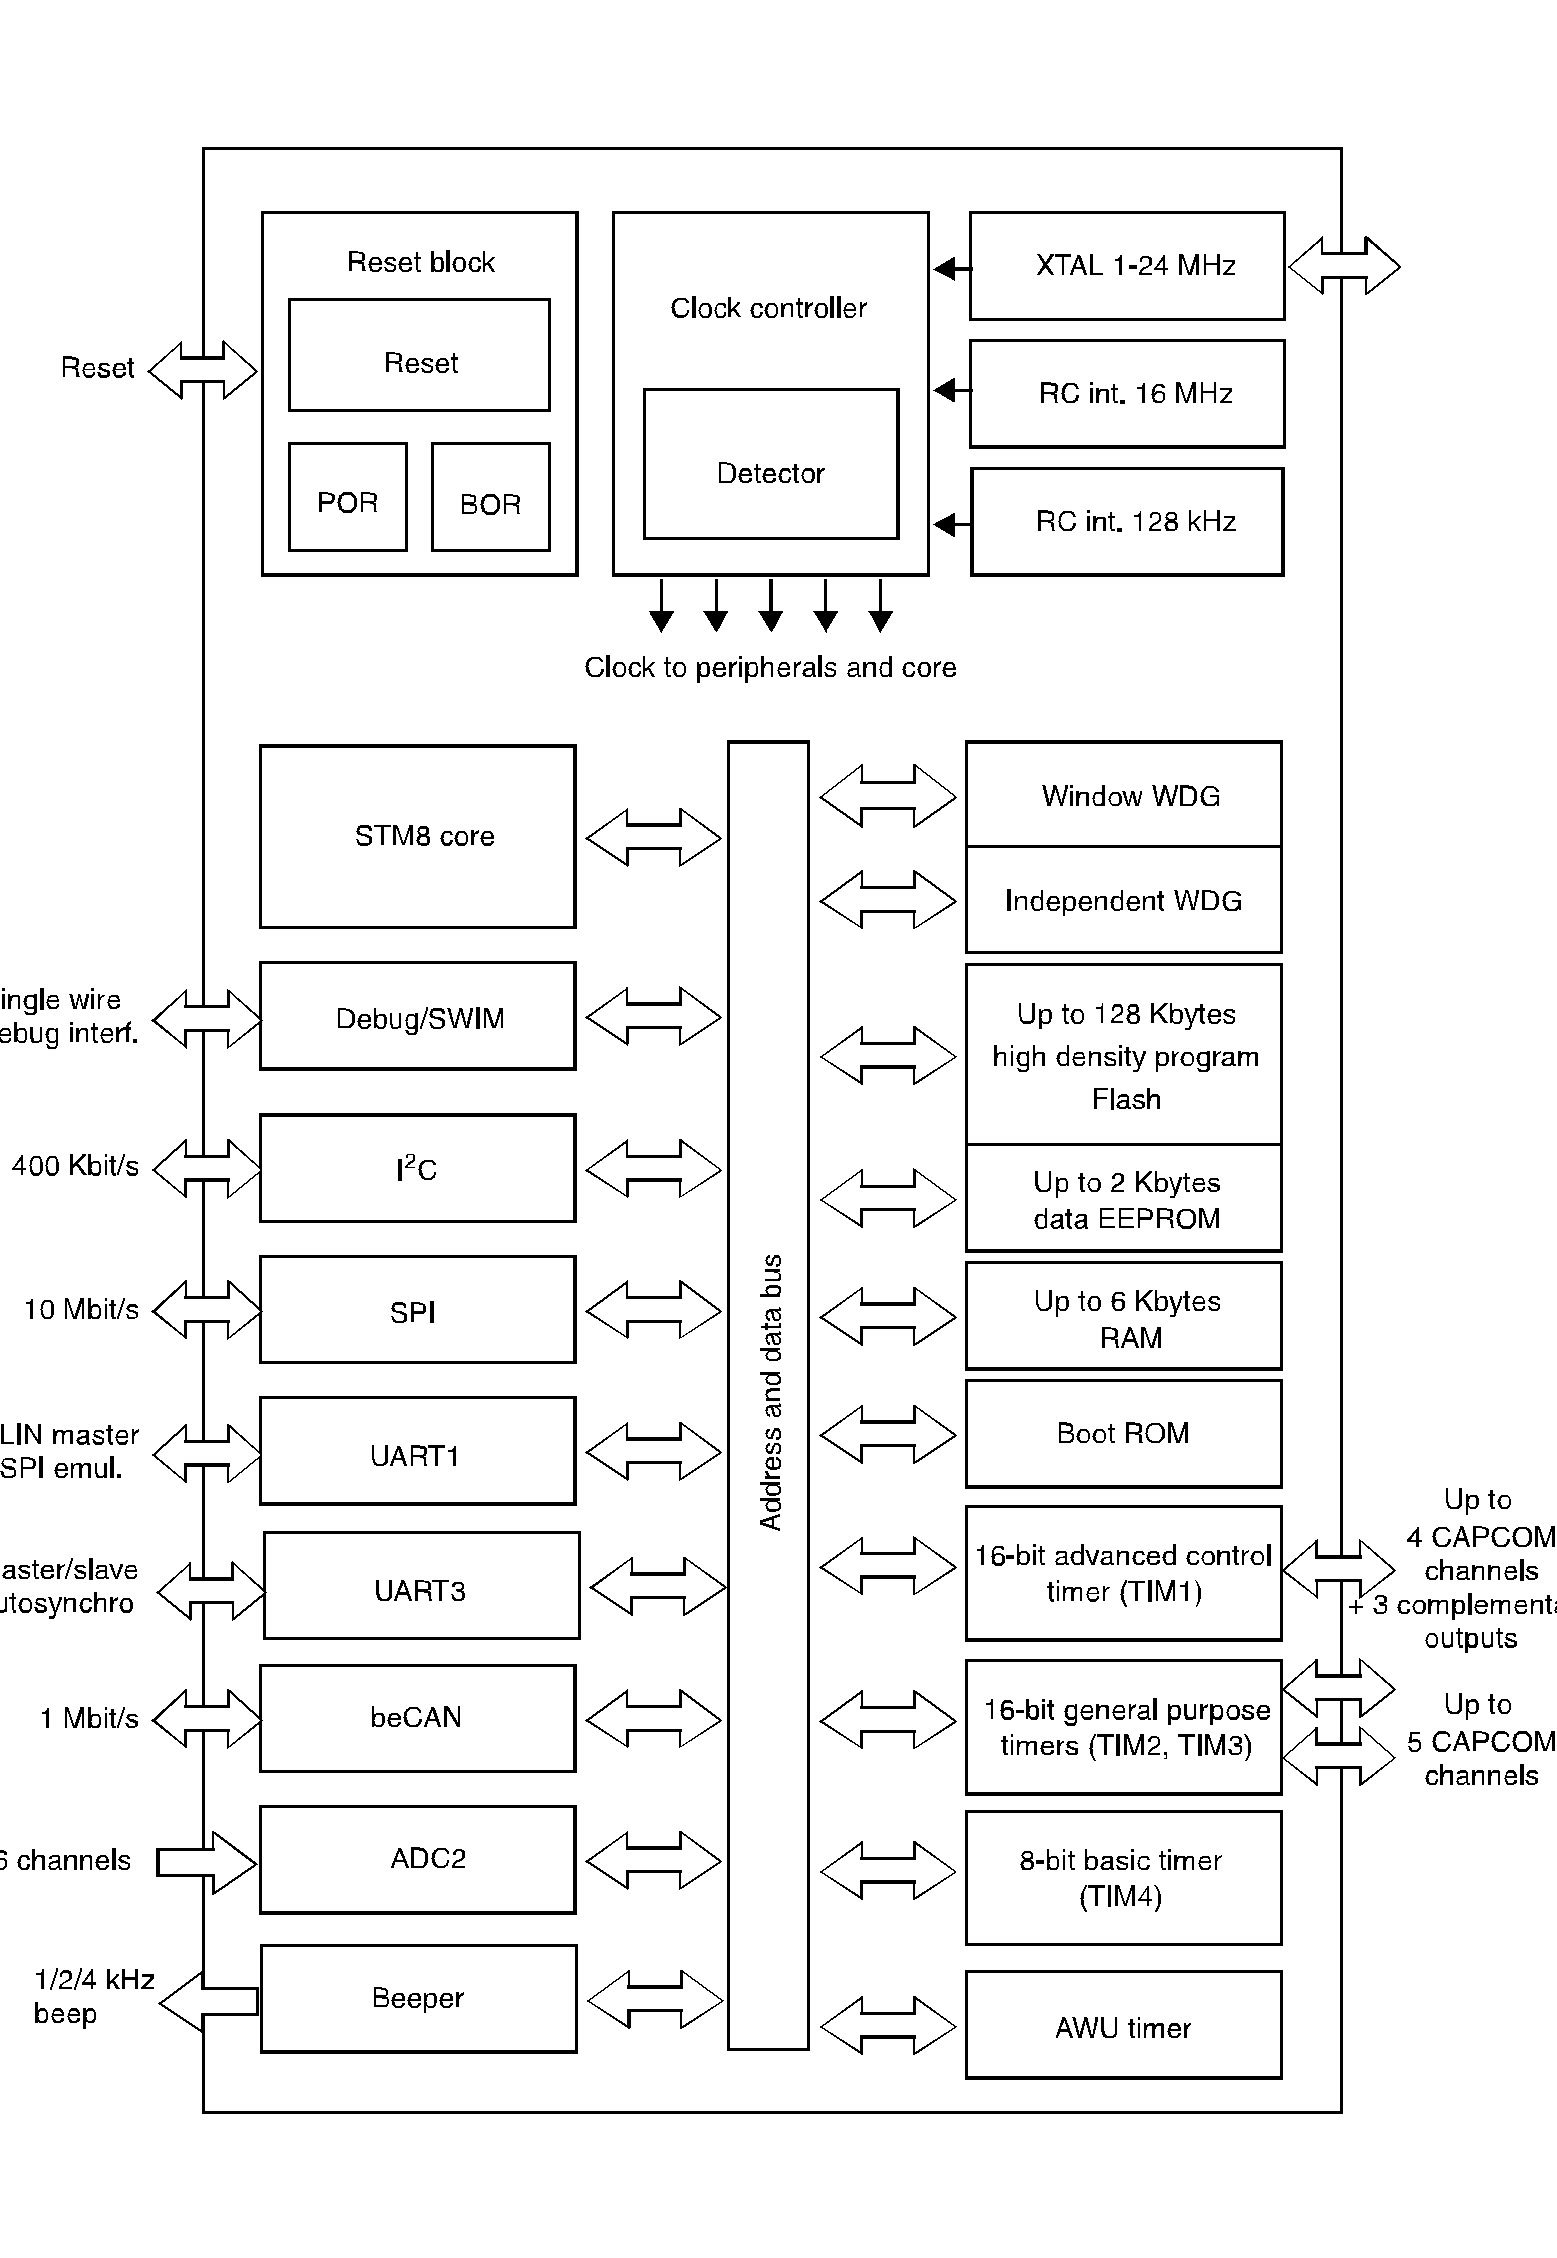
\includegraphics{figures/circuit_diagram.jpg}
\caption{芯片的电路图}
\end{figure}

\chap{STM8编程实战之基础篇}

本章从一个呼吸灯实验入手,再逐步加入中断、计时器等。带

\section{STM8官方库函数简介}

为了便于使用者快速开发程序,意法半导体公司为STM8开发了库函数,并带有详尽的使用文档和使用案例。这样一来程序 我们要找的库函数文件在\url{http://www.st.com/internet/com/SOFTWARE_RESOURCES/SW_COMPONENT/FIRMWARE/stm8_stdperiph_lib.zip}。这个库函数适用于STM8S以及STM8A的芯片

\section{使用STVP建立自己的工程文件}

这节写的比较纠结,因为IDE的东西,操作说得太絮叨了。如果可以的话,根据上节所讲的知识,自己试试看建立自己的工程文件吧。

\section{COSMIC编译器}

在这个案例开始前,我们必须要清楚STM8的时钟以及GPIO。

\section{时钟}

分为Fmaster、Fcpu

Master时钟源有四种选择:

*1-24MHz高速外加晶振震荡时钟源(HSE)

*低于24Mhz一个外加时钟频率信号(HSE user-ext)

*芯片自带的一个16MHz高速RC震荡时钟源(HSI)

*芯片自带的一个128KHz低速RC震荡时钟源(LSI)

默认情况下,系统默认使用HSI/8的时钟源,也就是说系统默认的运行速率是2Mhz。

\subsection{时钟树}

\section{GPIO}

\subsection{GPIO的几种状态}

\section{中断}

\section{计时器}

\chap{STM8编程实战之提高篇}

\section{USART}

\section{SPI}

\section{TWI}

\chap{STM8资源补遗}

\section{IWDG}

\section{WWDG}

\section{AWT}



\appendices
\renewcommand{\prechap}{\appendixname}
\renewcommand{\postchap}{}


\end{document}
